\scanpage{25}
\mspage{22}
La donnée d'une structure de réseau discret sur $L$ revient à celle d'une \deleted{structure} partie $S$ de $\mathcal P_2(L)$
[les axiomes F1) à F6) sont vides !]
donc une structure de \uline{graphe} réduit.

\begin{center}\rule{0.9cm}{0.7pt}\end{center}

[Je reviens à l'étude des réseaux réguliers \unsure{et} connexes (\inserted{et} non vides, i.e. 0-connexes)]

\deleted{Lemme}
On va étudier les cas de figure de deux segments ``consécutifs''

\margin{$\unsure{\mathcal R|R}$ quelconque avec $y$ \uline{régulier}}

\figure{\begin{tikzpicture}[x=1cm,y=1cm]
\draw (0,0)--(2.95,.13); \draw (3.25,.16)--(5.9,.35);
\draw (0,-.07)--(0,.07);
\fill (3.1,.15) circle(.035); \fill (5.9,.35) circle(.025);
\node[below] at (0,0) {$x$};
\node[below] at (3.1,.15) {$y$};
\node[below right] at (5.9,.35) {$z$};
\node[above] at (1.5,.08) {$I$};
\node[above] at (4.5,.24) {$J$};
\end{tikzpicture}}

avec \inserted{$y\in\delta I\cap\delta J$}, $\operatorname{br}_y(I)\ne\operatorname{br}_y(J)$, \inserted{$y\in L_r$}, Je distingue deux cas :

I) $I\cap J=\{y\}$ alors \deleted{\unsure{Si}} par axiome de recollement,
$\exists!K\in S$, $K\supset I\cup J$, $\delta K=\{x,z\}$,
et $I=K_{xy}$, $J=K_{yz}$. Situation bien comprise.

\deleted{II) $I\cap J\ne\{y\}$. \unsure{On distingue un} \inserted{Soit}

a) $x=z$

\deleted{\unsure{a)|ou} $I\cap J=\{y,x\}$}

\figure{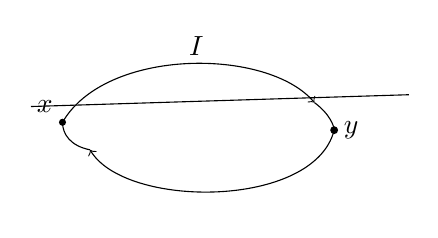
\begin{tikzpicture}[x=1cm,y=1cm]
\draw[->] (0,0) .. controls (.55,.95) and (2.6,.95) .. (3.2,.25);
\draw (3.2,.25) .. controls (3.4,.1) and (3.45,-.05) .. (3.45,-.1);
\draw[->] (3.45,-.1) .. controls (3.2,-1.1) and (.8,-1.1) .. (.35,-.35);
\draw (.35,-.35) .. controls (.1,-.3) and (0,-.15) .. (0,0);
\fill (0,0) circle(.045); \fill (3.45,-.1) circle(.05);
\node[above left] at (0,0) {$x$}; \node[right] at (3.45,-.1) {$y$};
\node[above] at (1.7,.72) {$I$};
\draw (-.4,.2)--(4.4,.35);
\end{tikzpicture}}

b) $I\cap J\ne\{y,x\}$ \unsure{si} $(x\ne y)$ \unsure{alors}

$\exists t\in I\cap J,\ t\ne y$.}
\mspage{24}

\rotatebox{90}{\reflectbox{\unsure{EXTRA STRONG}}}
\rotatebox{90}{\reflectbox{\unsure{EXTRA STRONG}}}
